\documentclass[12pt]{scrartcl}

	\author{\textbf{Benjamin Andrea Schüpbach}\\ \\Matr.No. 14-100-564\\benjamin.schuepbach@students.unibe.ch\\Master's Student in Geography\\Institute of Geography, University of Bern\\}
	
	\date{August 2019}
	
	\title{\textbf{ICARUS\\}}
	
	\subtitle{Lessons Learned from using Image Classification on Big Data to estimate an indicator of Sustainable Development\\}

	%Packages Used%
	\usepackage[utf8]{inputenc}
	\usepackage[round]{natbib}
	\usepackage{graphicx}






\begin{document}
	\maketitle
	\newpage
	
	
	
	\section{Introduction}
		
		\nocite{*}
		\subsection{Sustainable Development}
		
		
		
		\subsection{Development Disparities}
		
		
		
		\subsection{Big Data}
			\subsubsection{Big Data Analyses}
			
			\subsubsection{Big Data for Sustainability}
			
			\subsubsection{title}
			
			
			
		\subsection{Image Classification}
			\subsubsection{Deep Neural Networks}
			
			\subsubsection{YOLO \& Darkflow}
			
			\subsubsection{title}
			
			\subsubsection{title}
			
			
			
		\subsection{Goals of this Study}
			\subsubsection{Research Questions}

		

		

	
	\newpage
	\section{Methods}
	Introduce Methods by means of a flowchart!
		\subsection{Harvesting of training images}
		\subsection{Supervised Classification}
		\subsection{Training ICARUS}
		\subsection{Validation}
	
	\newpage
	\section{Results}
		\begin{figure}[h]
			\centering
			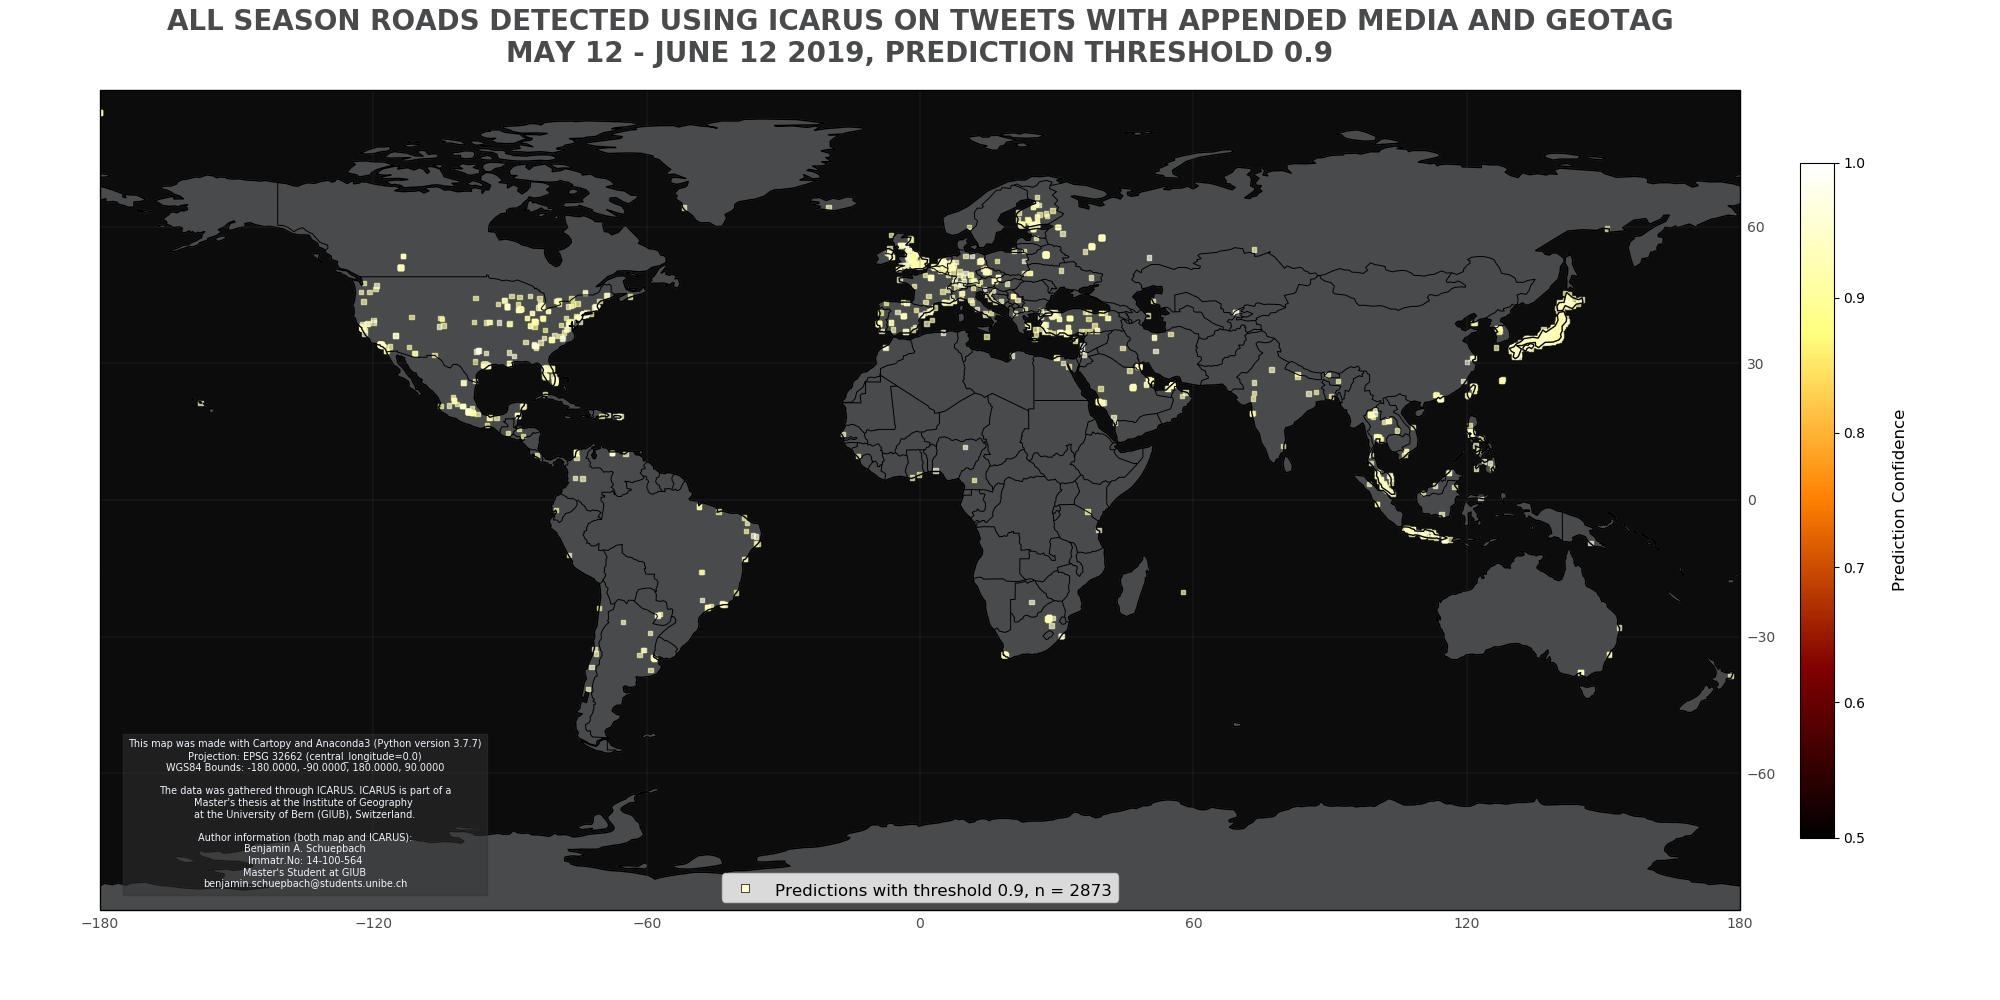
\includegraphics[scale=0.3]{images/map_ICARUS_thresh90}
			\caption{Figure 1: Map of Tweets where ICARUS identified AllSeasonRoads}
			\label{fig: 1}
		\end{figure}
	
	\newpage
	\section{Discussion}

	\newpage
	\section{Conclusion \& Outlook}
		\subsubsection{title}



	\newpage
	\bibliographystyle{plain}
	\bibliography{mybib}
\end{document}

